\documentclass{article}
\usepackage{calc}
\newlength{\pagewidth}\setlength{\pagewidth}{7.44in}
\newlength{\pageheight}\setlength{\pageheight}{9.69in}
\newlength{\spine}\setlength{\spine}{1.118in}
\newlength{\coverbleed}\setlength{\coverbleed}{.125in}
\newlength{\height}\setlength{\height}{\pageheight+2\coverbleed}
\newlength{\width}\setlength{\width}{2\pagewidth+2\coverbleed+\spine}
\usepackage[margin=0in,noheadfoot,paperwidth=\width,paperheight=\height]{geometry}
\pagestyle{empty}
\setlength{\parindent}{0in}
\usepackage{tikz}
\begin{document}
\begin{tikzpicture}[x=1in,y=1in]
\clip (0,0) rectangle (\width,\height);
\node[anchor=south west] at (\coverbleed,\coverbleed) {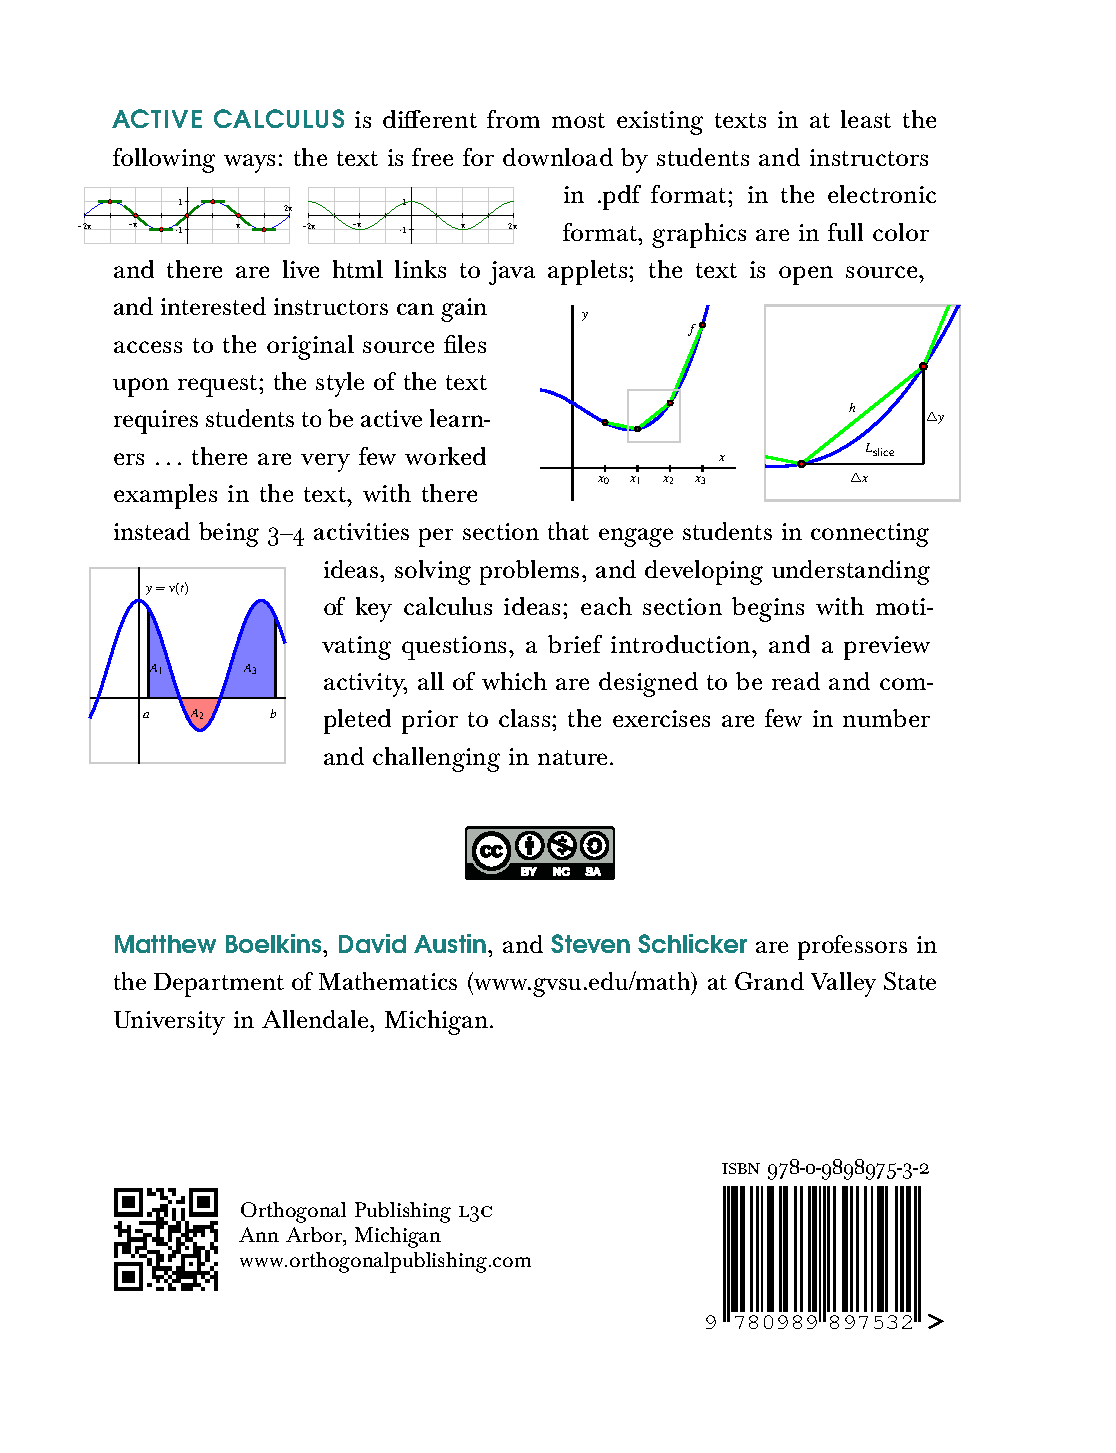
\includegraphics{backcover.pdf}};
\node[anchor=south west] at (\coverbleed+\pagewidth+\spine,\coverbleed) {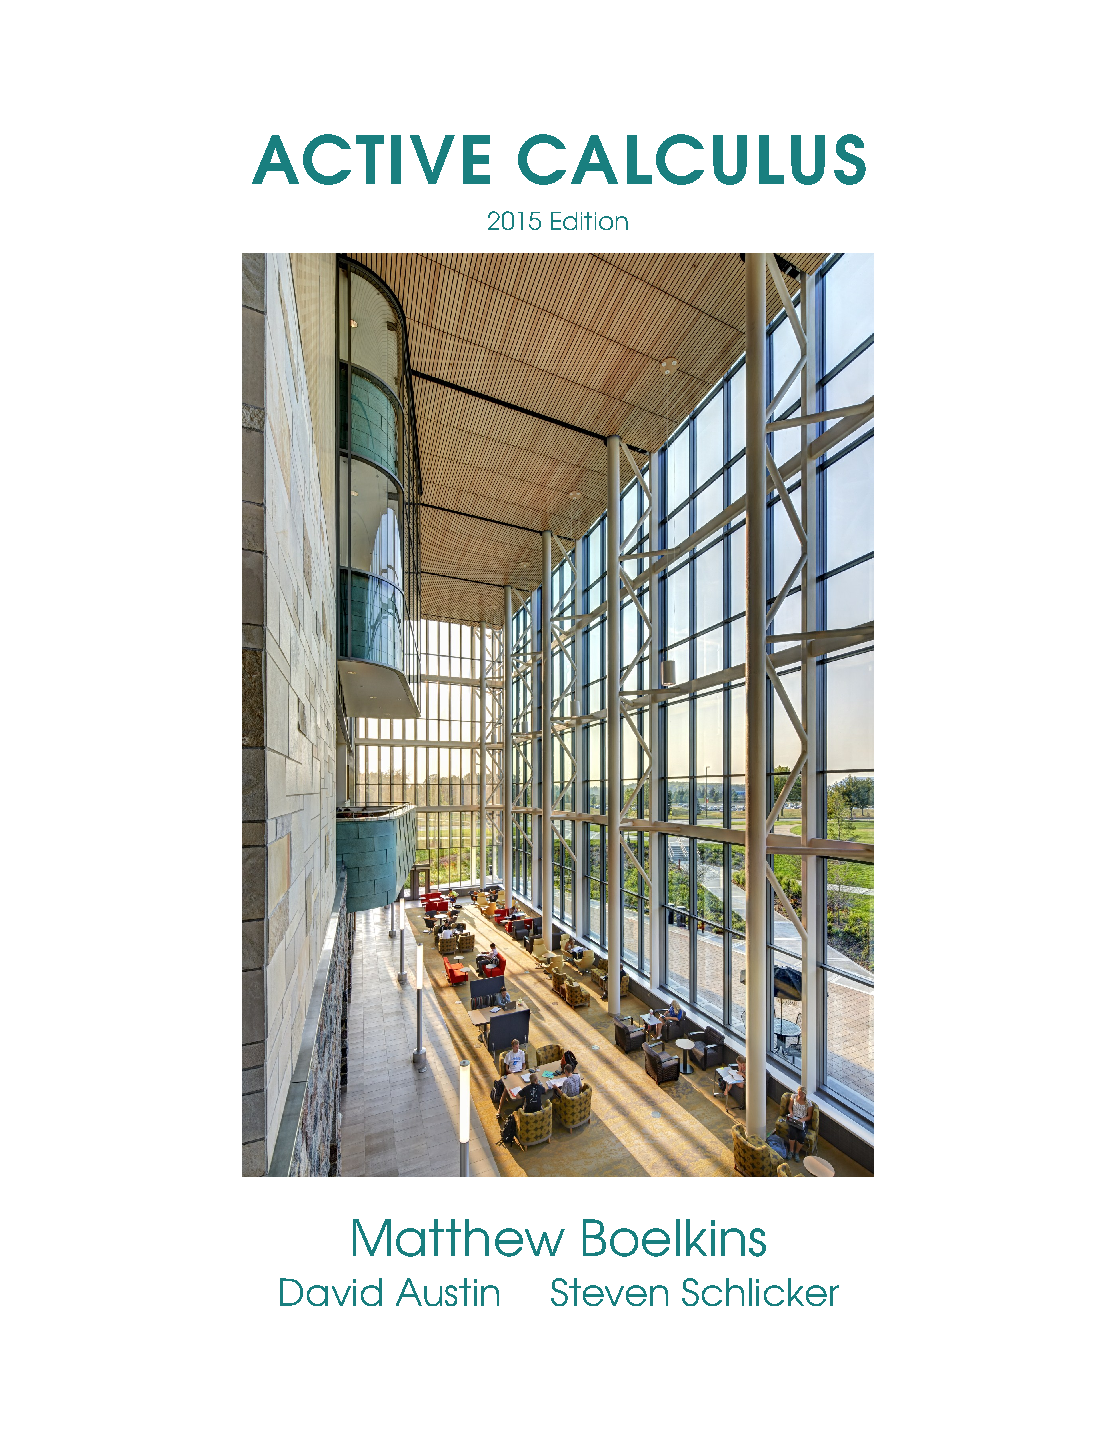
\includegraphics{frontcover.pdf}};
\node at (\coverbleed+\pagewidth+.5\spine,\coverbleed+.5\pageheight) {\rotatebox{270}{
\includegraphics{spine.pdf}}} ;
\end{tikzpicture}
\end{document}